% TODO vind meer sources
\chapter{Software Engineering}
The Institute of Electrical and Electronics Engineers \texttt{[IEEE]} defines the practice of Software Engineering as: "Application of a systematic, disciplined, quantifiable approach to the development, operation and maintenance of software; that is, the application of engineering to software" \cite[p.~421]{8016712}. The word ``systematic'' in this definition, emphasises the need for a structured process, depicting guidelines and models that describe how software should be developed the most efficient way possible. Such a process does exist and it is often referred to as the Software Development Life Cycle (SDLC) \cite[p.~420]{8016712}. 

\section{Software Development Life Cycle}
An implementation of the SDLC consists of two major components. First, the process is broken down into several smaller phases. Depending on the nature of the software, it is possible to omit steps or add more steps. I have compiled a simple yet generic approach from multiple sources \cite{2010govardhan}, to which most software projects adhere. This approach consists of five phases.
\begin{enumerate}
	\bolditem{Requirements phase} This is the initial phase of the development journey. During this phase, the developer gets acquainted with the project and gathers information about the requested features. Based upon this, the developer eventually decides on the required hardware specifications and possible external software which will need to be acquired.
	\bolditem{Design phase} After the developer has identified the features, they can use this to draw an architectural design of the application. This design consists of multiple documents, including user stories and UML diagrams.
	\bolditem{Implementation phase} During this phase, the developer will write code according to the specifications of the architectural designs.
	\bolditem{Testing phase} This is the most important phase. During this phase, the implementation is tested to identify potential bugs before the application is used by other users.
	\bolditem{Operational phase} In the final phase, the project is fully completed and it is integrated in the existing business environment.
\end{enumerate}

\noindent Subsequently, a model is chosen to define how to transition from one phase into another phase. A manifold of models exist \cite{2010govardhan}, each having advantages and disadvantages, but I will consider the basic yet most widely used model, which is the Waterfall model by Benington \cite{united1956symposium}. The initial Waterfall model required every phase to be executed sequentially and in order, cascading. However, this imposes several issues, the most prevalent being the inability to revise design decisions taken in the second phase, when performing the actual implementation in the third phase. To mitigate this, an improved version of the Waterfall model was proposed by Royce \cite{Royce:1987:MDL:41765.41801}. This version allows a phase to transition to a previous phase, as illustrated in \autoref{fig:waterfall-royce}.

\begin{figure}[htbp!]
	\centering
	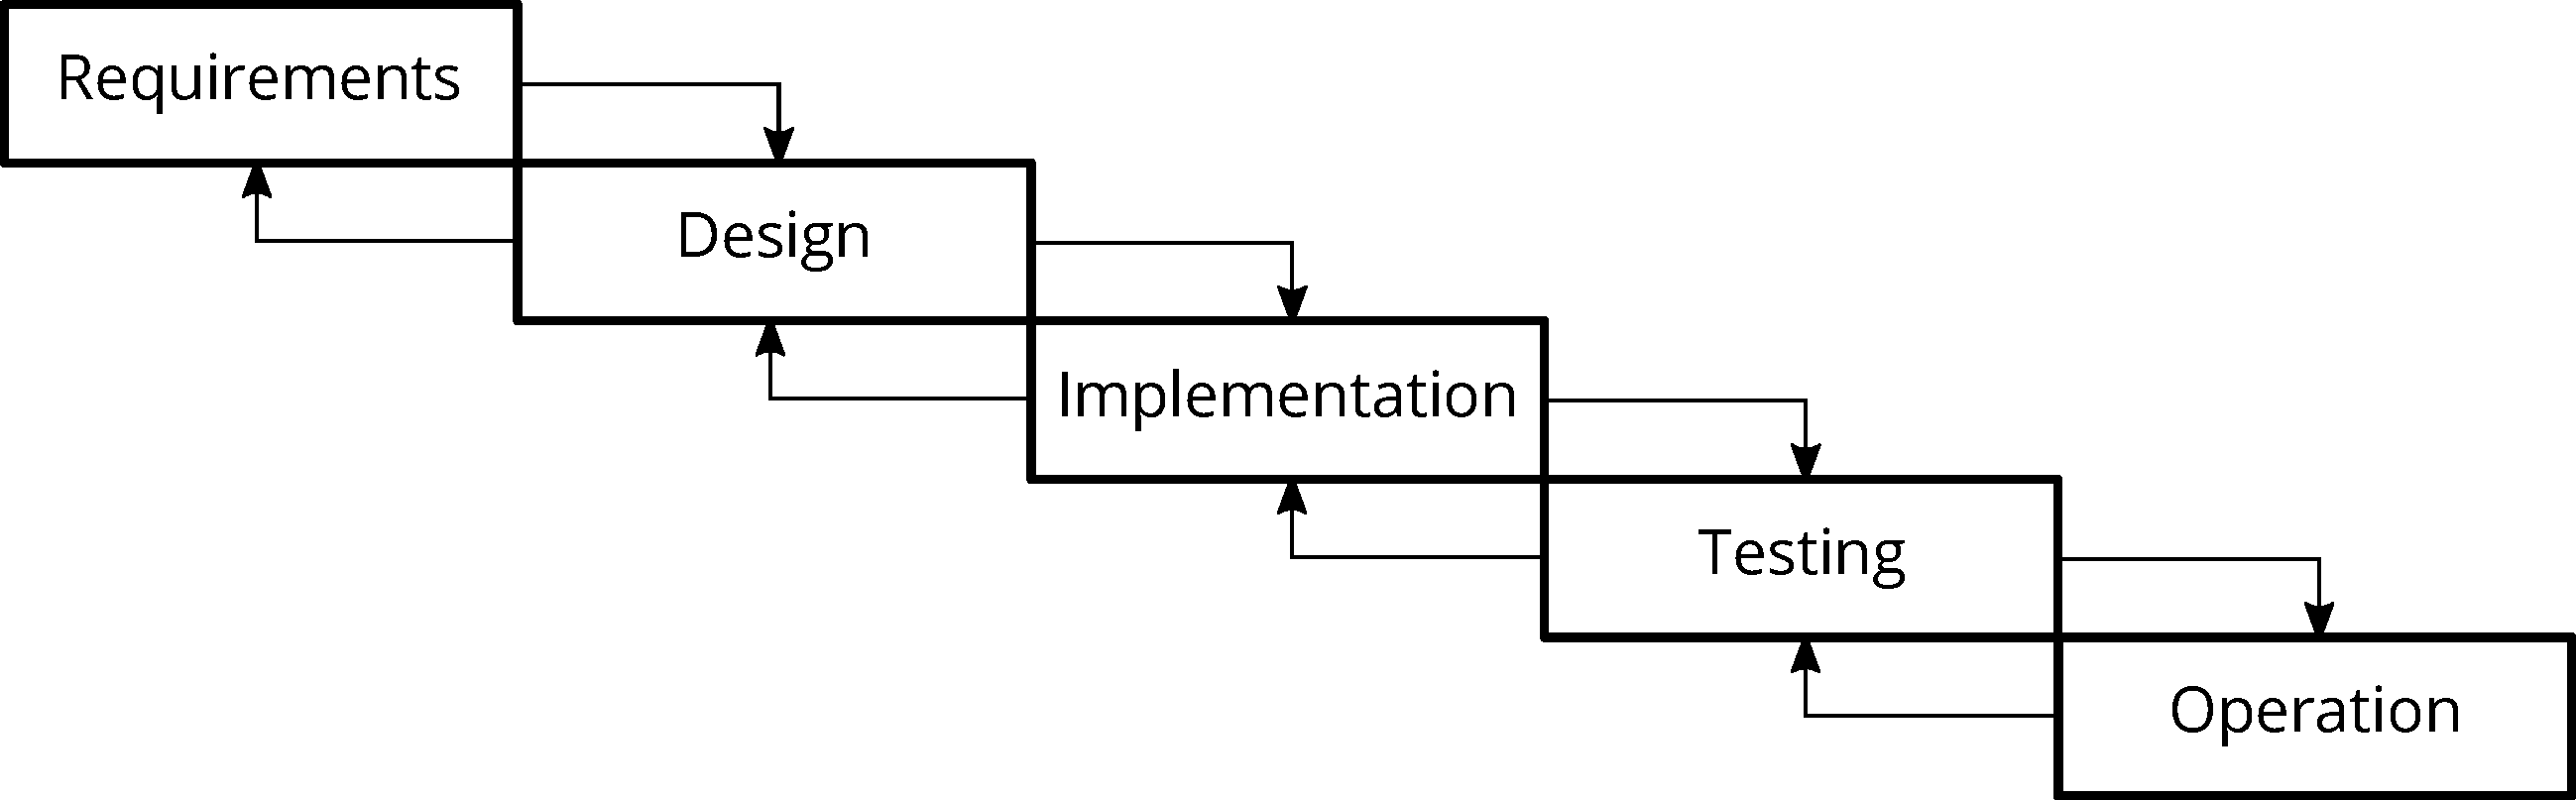
\includegraphics[width=\textwidth]{assets/sdlc.pdf}
	\caption{Improved Waterfall model by Royce}
	\label{fig:waterfall-royce}
\end{figure}

\noindent In this thesis I will solely focus on the implementation and testing phase, as these are the most time-consuming phases of the entire process. The modification to the Waterfall model by Royce is particularly useful when applied to these two phases, in the context of \emph{software regressions}. A regression \cite{10.1007/978-3-540-77966-7_18} is a feature that was previously working correctly, but is now malfunctioning. This behaviour can have external causes, such as a change in the system clock because of daylight saving time, but can also be the result of a change in the code of another, seemingly unrelated, part of the software component.\\

\noindent Software regressions and other functional bugs can ultimately lead to disastrous effects, such as severe financial loss or damage to the reputation of the software company. The most famous example in history is without any doubt the explosion of the Ariane 5-rocket, caused by an integer overflow \cite{581900}. In order to reduce the risk of bugs, malfunctioning components should be detected as soon as possible to proactively defend against potential failures. Because of this reason, the testing phase is to be considered as the most important phase of the entire development process and an application should include a plethora of tests. The set of all tests, or a smaller chosen subset of certain tests of an application is referred to as the \emph{test suite}. This thesis considers three distinguishable categories:

\begin{enumerate}
	\bolditem{Unit test} This is the most basic kind of test. The purpose of a unit test is to verify the behaviour of an individual component \cite{whittaker2000}. The scope of a unit test is typically limited to a small and isolated piece of code, such as one function.
	\bolditem{Integration test} A more advanced test, an integration test verifies the interaction between multiple individually tested components \cite{whittaker2000}. Examples of integration tests include the communication between the front-end and the back-end side of an application.
	\bolditem{Regression test} After a regression has been detected, a regression test \cite[p.~372]{8016712} is added to the test suite. This test aims to replicate the exact conditions and sequence of actions that have caused the regression, in order to warden the implementation against subsequent failures in the future.
\end{enumerate}

\noindent A frequently used metric to measure the quantity and effectiveness and thoroughness of a test suite is the \emph{code coverage} or \emph{test coverage} \cite[p.~467]{8016712}. The test coverage is a percentage that indicates which fraction of the application code is affected by code in the test suite. Internally, this works by augmenting every statement in the application code using binary instrumentation. A hook is inserted before and after every statement to keep track of which statements are executed during tests. Many different ways exist to interpret these instrumentation results and thus to calculate represent the fraction of covered code:

\begin{itemize}
	\bolditem{Line coverage} (TODO explain + sources)
	\bolditem{Statement coverage} (TODO explain + sources)
	\bolditem{Branch coverage} (TODO explain + sources)
\end{itemize}

It should be self-evident that achieving, and maintaining, a coverage percentage of 100\% at all times is critical. However, this does not necessarily imply that all lines, statements or branches need to be covered \cite{dein_2019}. All major programming languages have frameworks and libraries available to collect coverage information during test execution. The most popular options are JaCoCo\footnote{\url{https://www.jacoco.org/jacoco/}} for Java, coverage.py\footnote{\url{https://github.com/nedbat/coveragepy}} for Python and simplecov\footnote{\url{https://github.com/colszowka/simplecov}} for Ruby. These frameworks are able to generate in-depth statistics on which parts of the code are covered and which parts require more tests, as illustrated in \autoref{fig:coverage-statistics}.

\begin{figure}[htbp!]
	\centering
	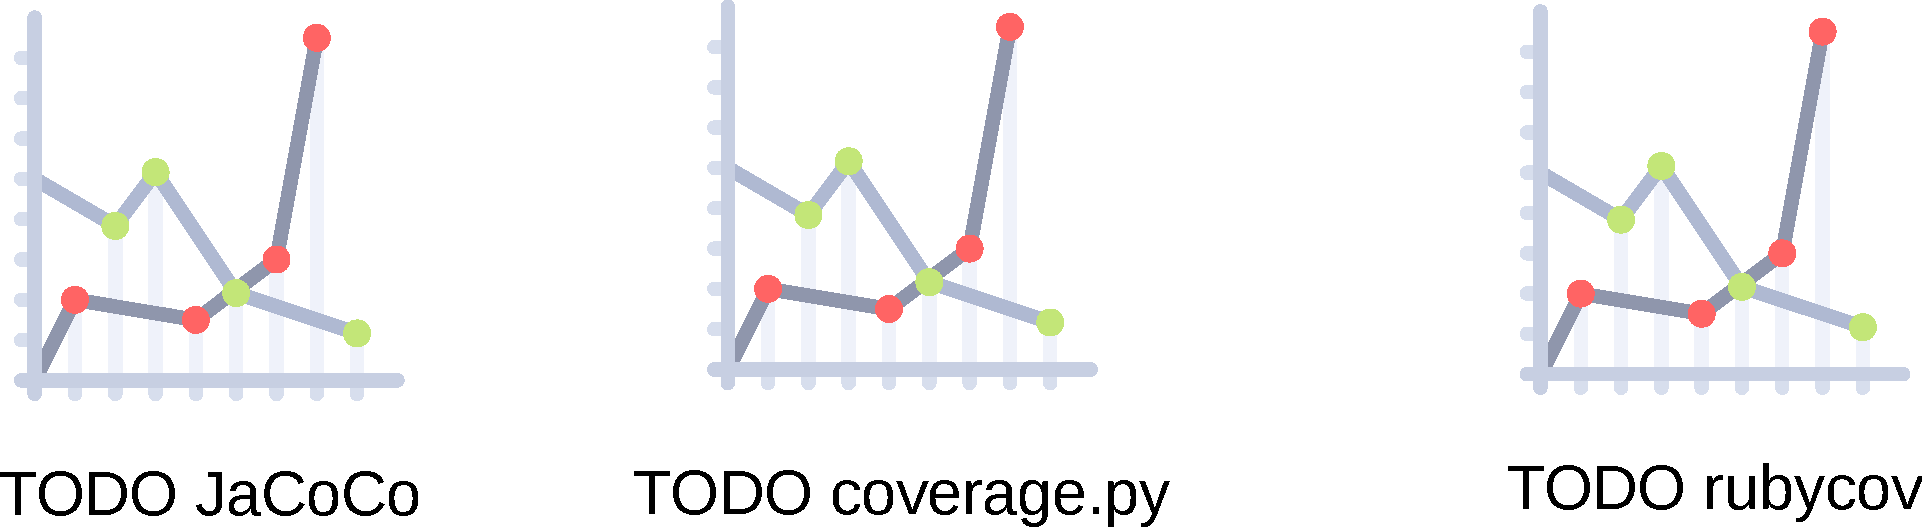
\includegraphics[width=\textwidth]{assets/coverage.pdf}
	\caption{Statistics from Code coverage tools}
	\label{fig:coverage-statistics}
\end{figure}

\section{Continuous Integration}

Over the past decade, following the financial crisis of 2009 \cite{ionel2009}, extensive research has been put into reducing the time occupied by the implementation and testing phases. This resulted in a new development approach, known as \emph{Agile programming} \cite{torgeir2010}. The main philosophy of Agile programming is that the time-to-market should be as short as possible, allowing end-users to provide feedback much earlier in the process. (TODO)

- waarom

- wat

- voorbeelden: Jenkins, CircleCI, Travis-CI, recent GitHub Actions + screenshots

- Probleem en oplossingen met regression tests

  - Test Case Prioritization -> Focus want geen tests weggooien
  
  - Test Suite Minimization
  
  - Test Suite Selection
  
  - Test Suite Reduction
